\documentclass[thesis.tex]{subfiles}
\begin{document}
The content of the previous chapter allow us to easily implement the equilibrated flux estimator, and present some (interesting) results.
We will analyze the unknown constants present in the error bounds using this implementation.
In particular we seek out to answer questions like: How tight is the error bound given by the equilibrated flux estimator?
What is the practical convergence rate of AFEM driven by the equilibrated flux estimator?
How do the equilibrated flux estimator and classical estimator --- both optimal AFEM drivers --- compare to eachother?


  MATLAB \cite{MATLAB:2015} is  used for the actual implementation. We 
  make extensive use of iFEM~\cite{chenifem}, a Matlab framework for (adaptive) finite element methods. 
  All of the results are gathered for the \emph{linear} lagrange finite element space $\VV(\T)$.
  We let iFEM  calculate the linear discrete solution $U$ for a given partition.
  The package ships with an implementation of the \emph{newest vertex bisection} refinement algorithm.
  This refinement method bisects triangles and ensures conformity as well as shape regularity of the resulting triangulation.
  We will first asses some (normal) finite element solutions.  After this we will
  consider the performance of the adaptive finite element method driven by the (lowest order) equilibrated flux estimator. The results
  will be compared to the classical residual estimator. The implementation calculates $\vzet$ from \eqref{eq:systemzeta} and uses the element-wise estimator from Theorem~\ref{thm:zetaupper}.

  \section{Exact error}

  For meaningful results we ideally compare our error bounds from Theorem~\ref{thm:zetaupper} to the \emph{exact} error $\enorm{u - U}_\O$. Unfortunately this is
  not possible in most situations. If one knows the exact solution $u$ of an interesting problem, then
  the right hand side $f$ of the associated Poisson problem is almost never constant, rendering our implementation useless. 
  We have two ways to overcome this problem. 
  
  The first is to treat the $f$ as if it was piecewise constant; that is, 
  we approximate $\ip{\psi_a f - \nabla \psi_a \nabla U, q_k}_K$ by the edge-midpoint quadrature and ignore this approximation error. Similarly we simply replace the
  data oscillation term $\uanorm{f - \div \v{\zeta}}_K$  by its edge-midpoint quadrature. Provided that $f$ is sufficiently smooth, the effects of these extra errors are of higher order $h$, and thus should be insignificant for small diameter.
  
  The other approach is using a constant $f$, without knowing the exact solution $u$. We propose to approximate the true error $\enorm{u - U}_\O$ by replacing $u$ with another finite element solution $U_\star$  --- quite dazzling if one thinks about it.
  To make this work we let~$U_\star$ be a solution on a finer triangulation $\T_\star \geq \T$, such that
  every element in $\T_\star$ is at least \emph{one} bisection away from its corresponding element in $\T$. We have
  \[
    \enorm{u - U}_\O \leq \uaenorm{u - U_\star}_{\O} + \uaenorm{U - U_\star}_{\O},
  \]
  where we hope --- which is most likely the case if $u$ possesses some smoothness --- that 
  $\uanorm{u - U_\star}_{\O} \ll \uanorm{U - U_\star}_{\O}$. 
  An straightforward implementation of this approximation follows from noting that $U$ lies in the finite element spaces $\VV(\T_\star)$
  for refined triangulations $\T_\star \geq \T$.  iFEM  conveniently provides a function that calculates the
  coefficients of $U$ with respect to the linear basis of $\T_\star$.
  \section{Uniform refinements}
  First we calculate the normal finite element solutions: we let iFEM calculate
  the linear discrete solutions $(U_k)_{k \geq 0}$ for a sequence of uniformly bisected triangulations $(\T_k)_{k \geq 0}$, 
  i.e. every triangle is bisected into four subtriangles. We then compare the estimators on this produced sequence of triangulations
  and discrete solutions.
  \begin{exmp}[Unit square]
    \label{ex:squaresin}
  Take $\O = (0,1)\times(0,1)$ with exact solution $u(x,y) = \sin(2\pi x)\sin(2\pi y)$, and thus
  \begin{equation*}
    \begin{alignedat}{2}
      -\Delta u &= 8\pi^2\sin(2\pi x)\sin(2\pi y)  \quad &&\text {in } \Omega, \\
      u &= 0 \quad &&\text{on } \partial\O.
    \end{alignedat}
  \end{equation*}
\end{exmp}
  The exact solution has four peaks and is very smooth. iFEM uses third order quadrature to approximate the integrals containing $f$.
  The produced discrete solutions $U_k$ are illustrated in Figure~\ref{fig:squareuh}.
  \begin{figure}
    \centering
    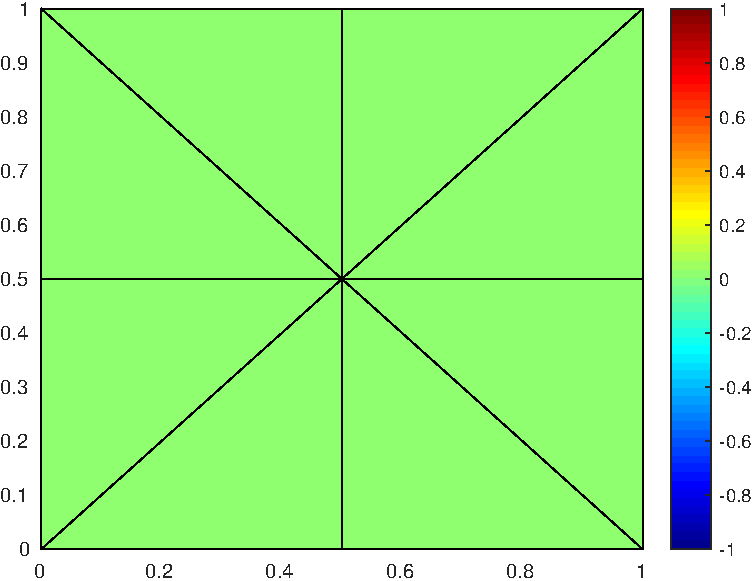
\includegraphics[width=.32\linewidth]{square_sin/mesh_uh_1.pdf}
    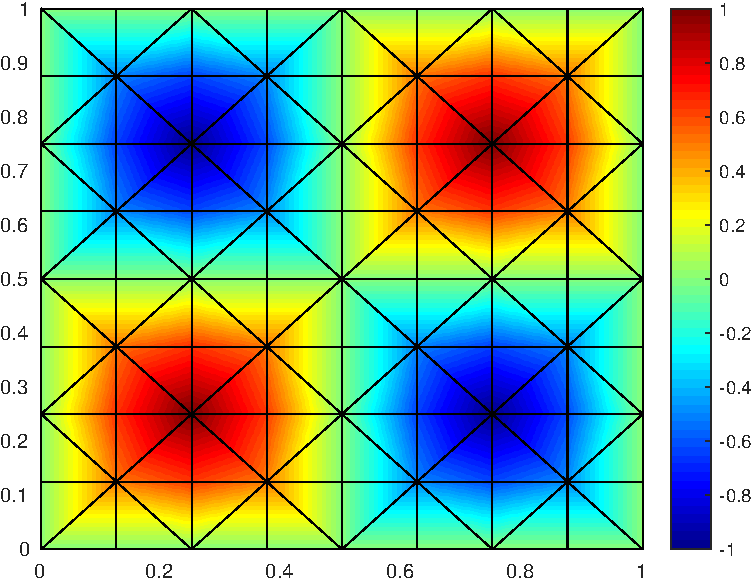
\includegraphics[width=.32\linewidth]{square_sin/mesh_uh_3.pdf}
    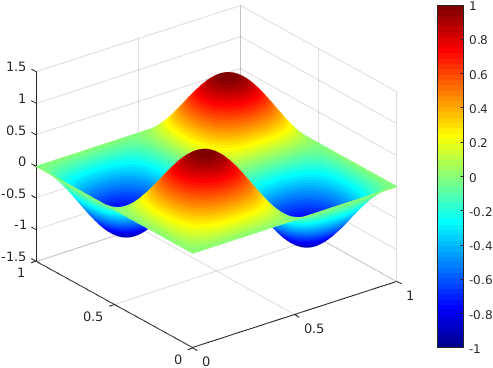
\includegraphics[width=.32\linewidth]{square_sin/result_uh_8.png}
    \caption{The finite element solutions $U_k$ for Example~\ref{ex:squaresin} with  uniformly bisected triangulations, from left to right we have diameters $h = 2^{-1}, 2^{-3}, 2^{-8}$.}
    \label{fig:squareuh}
\end{figure}
The images clearly visualize some convergence of the FEM solution. 
As $u \in H^2(\O)$ we expect that $\enorm{u - U_k}_{\O} \lesssim h \abs{u}_{H^1(\O)}$. For uniform refinements this
latter is equivalent to $\enorm{u - U_k}_{\O} \lesssim N^{1/2} \abs{u}_{H^1(\O)}$, with $N$ the total number of vertices.

The iFEM package provides a method to calculate $\enorm{u - U}_{\O}$ given the exact $u$, 
and also provides an implementation of the standard residual estimator $\hat \eta_\T(U, \T)$.
We compare these against the equilibrated flux estimator from Theorem~\ref{thm:zetaupper},  i.e.
\[
  \enorm{u - U}_{\O} \leq \sqrt{\sum_{K \in \T} \eta^2_\T(U, K)} \quad \text{with} \quad \eta^2_\T(U,K) :=  \left[ \uanorm{\vzet + \nabla U}_{K} + \frac{h_K}{\pi} \uanorm{ f - \div\v{\zeta}}_{K}\right]^2.
\]
We calculate the efficiency indices of these estimators as $\enorm{u - U_k} / \eta$. In the equilibrated flux case we would like this
value to be close to one, as this shows tightness of the estimator. 
In the residual case we have an extra constant in the reliability bound, and thus tightness depends also depends on this (unknown)
constant.
The results are given in Figure~\ref{fig:squareerror}. The experimental convergence rate is in line with the theoretical convergence 
rate, as can see using the slope triangle.
\begin{figure}
  \centering
  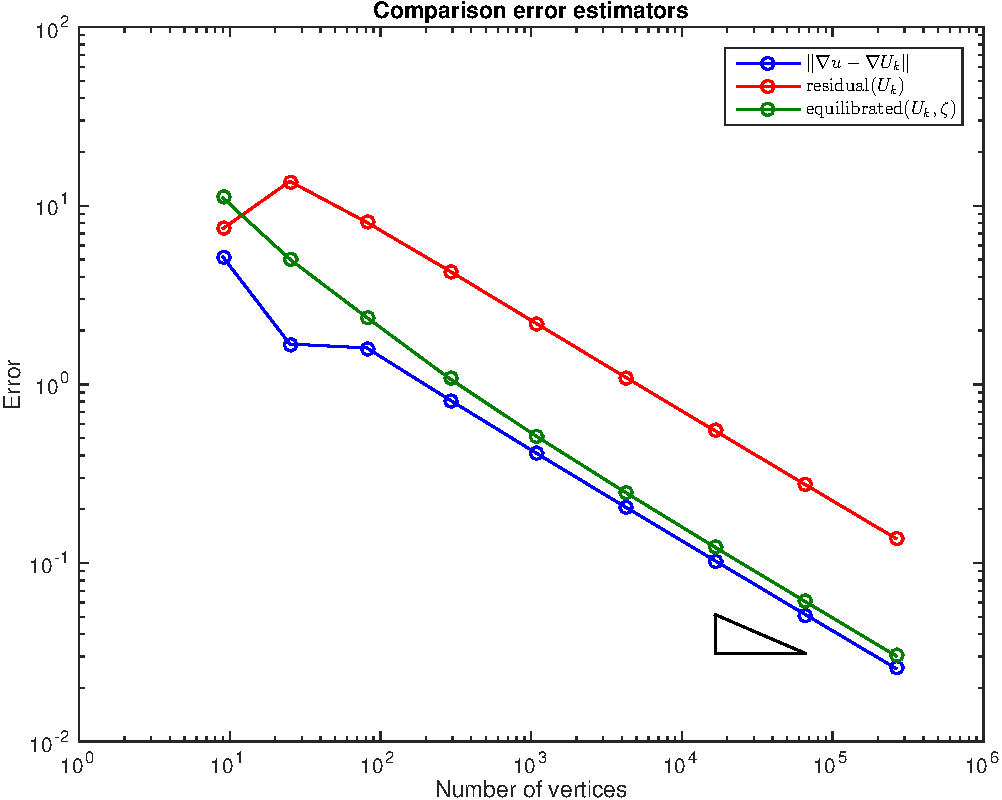
\includegraphics[width=.49\linewidth]{square_sin/norm_slope_9.pdf}
  \includegraphics[width=.49\linewidth]{square_sin/efficiency_9.pdf}
  \caption{The left compares the exact error in the energy norm with the standard residual estimator and the equilibrated flux estimator.  The results are gathered for discrete solutions $U_k$ of Example~\ref{ex:squaresin} using a sequence of uniformly refined triangulations.  The triangle has a slope of $-1/2$.  
  The right figure plots $\enorm{u - U_k} / \eta$; an estimation of the efficiency index.}
  \label{fig:squareerror}
\end{figure}

Even though we calculated the equilibrated flux estimator for $p=0$, it still proves to be real close to the actual error. The efficiency index
seems to increase, which could be explained by a reduction  of quadrature errors for smaller diameters. We have the exact solution
$u$ for this system, and thus we can empirically verify the claim that $\enorm{u - U_k}_{\O}$ is more or less equal to $\enorm{U_{k+i} - U_k}_{\O}$ for $i\geq 1$. A comparsion for  $i=1,2,3$ is given in Figure~\ref{fig:squareapprox}. The quality
of the error approximation increases with~$i$ as expected. 
\begin{figure}
  \centering
  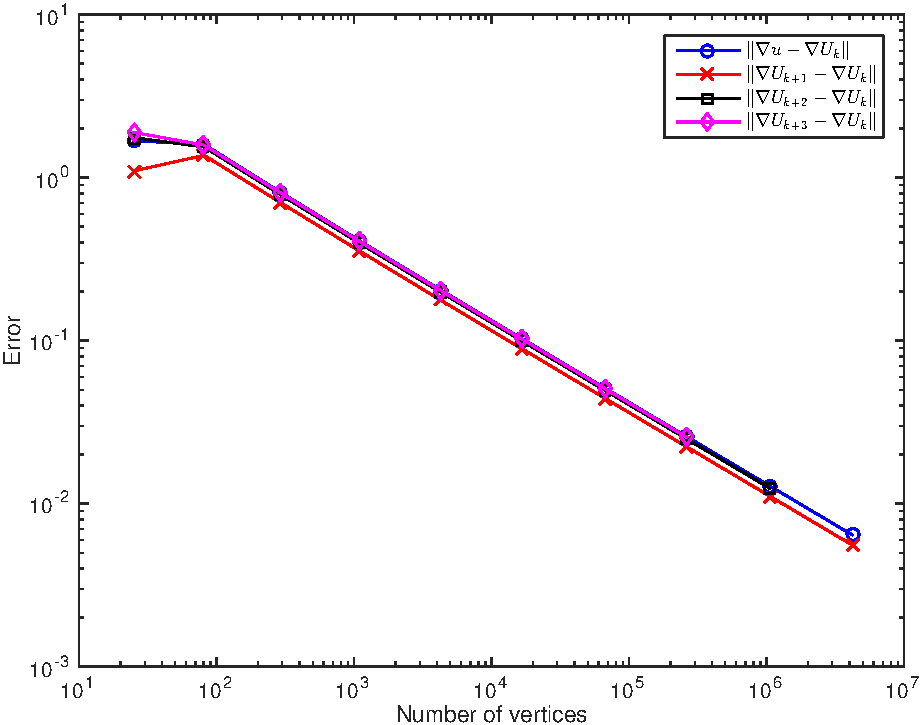
\includegraphics[width=.49\linewidth]{square_sin/approx_H1_10.pdf}
  \includegraphics[width=.49\linewidth]{square_sin/approx_H1_rel_10.pdf}
  \caption{ A comparision for Example~\ref{ex:squaresin} of the exact error $\enorm{u - U_k}_{\O}$ with the approximation $\enorm{U_{k+i} - U_k}_{\O}$ ($i=1,2,3$). In the left image all these norms are plotted, which results in a cluttered image as expected.
    The right image
  displays the relative terms, i.e. $\enorm{U_{k+i} - U_k}_{\O} / \enorm{u - U_k}_{\O}$.}
  \label{fig:squareapprox}
\end{figure}


\begin{exmp}
  \label{ex:squareana}
Another Poisson problem for the unit square domain is given by 
\[
  u(x,y) = 2^{40}x^{10}(1-x)^{10}y^{10}(1-y)^{10}.
\]
\end{exmp}
The corresponding right hand side $f$ is a high order polynomial; we let Matlab derivate  it using symbolic calculations. The
solution $u$ has a peak of value $1$ centered around $(\frac{1}{2}, \frac{1}{2})$ and is again very smooth. In Figure~\ref{fig:squareana}
the efficiency indices are given, alongside the relative errors generated by $\enorm{U_{k+i} - U_k}_{\O}$ for this new problem. The 
initial triangulation~$\T_0$ is equal the one used in the previous problem.
The efficiency of the equilibrated flux estimator is less for this problem, which is most likely due to the large oscillation factor,
but it still outperforms the classical residual estimator. 

The behaviour of $\enorm{U_{k+i} - U_k}_\O$ is very similar to that of the previous problem; it appears to be a good estimation of
the exact error $\enorm{u - U_k}_{\O}$.
In the following problems we will use this approximation,  due to the absence of an exact solution. 
For accuracy reasons we pick $i=3$, which should be enough for a `true error' indication.
We will write $U_{\star,k}$ for the discrete solution on $\T_{\star,k}$,
the triangulation found by uniformly refining every triangle in $\T_k$ three times.

\begin{figure}
  \centering
  \includegraphics[width=.49\linewidth]{square_ana/efficiency_9.pdf}
  \includegraphics[width=.49\linewidth]{square_ana/approx_H1_rel_10.pdf}
  \caption{Left image compares the efficiency indices of the standard residual estimator with the equilibrated flux estimator. Right image
  shows the exact error approximation quality. Results are gathered for Example~\ref{ex:squareana}.}
  \label{fig:squareana}
\end{figure}

\begin{exmp}[Re-entrant corner]
  \label{ex:lshape}
Here $\O = (-1,1)^2\setminus[-1,0]^2$ with right hand side $f = \1$; this is also known as the L-shaped domain. 
The solution $u$ of this problem has a singularity at the origin so
that $u \not \in H^2(\O)$. The theoretical
convergence on uniform refined triangulations is of order $h^{2/3}$.
\end{exmp}
 We calculate  discrete solutions $U_k$ for uniform refinements, and use $\uaenorm{\wt U_k - U_k}_\O$ to approximate the true error. 
The results are given in Figure~\ref{fig:lshapeone}. The experimental
convergence of the fem solution appears to match the theoretical convergence. 
The equilibrated residual once again has a better efficiency index than the residual estimator.
There is a drop in terms of efficiency compared to the previous problems. Interestingly, the efficiency of the equilibrated
estimator seems to decrease, whereas the efficiency of the standard estimator is somewhat increasing. 
This might be related to the approximation quality of $\uaenorm{\tilde U_k - U_k}_{\O}$.

\begin{figure}
  \centering
  \includegraphics[width=.49\linewidth]{lshape_one/norm_slope_8.pdf}
  \includegraphics[width=.49\linewidth]{lshape_one/efficiency_8.pdf}
  \caption{Error estimators and their efficiency for the re-entrant corner problem (Example~\ref{ex:lshape}). The triangle has a slope of $-1/3$.}
  \label{fig:lshapeone}
\end{figure}

\begin{exmp}[Crack domain]
  \label{ex:crack}
A problem with a line singularity is given by the crack domain: take $f = \1$ and
\[
  \O=\{(x,y) \in \R^2 : |x|+|y|<1\}\setminus ([0,1] \times \set{0}).
\]
The exact solution $u$ can be given in polar coordinates, $u(r, \phi) = r^{1/2}\sin(\phi/2) - 1/2 r^2 \sin^2 (\phi)$.
The theoretical convergence rate of uniformly refined triangulations is of order $h^{1/2}$, due to its line singularity. 
\end{exmp}

This
domain is implemented by adding the vertex $(1,0)$ twice.  
The results are given in Figure~\ref{fig:crackone}.
There is a drop in the efficiency index compared to the re-entrant corner; this could
be explained by the fact that $u$ is less regular. Again the efficiency of the equilibrated flux estimator decreases, while the efficiency
of the residual estimator increases.
\begin{figure}
  \centering
  \includegraphics[width=.49\linewidth]{crack_one/norm_slope_8.pdf}
  \includegraphics[width=.49\linewidth]{crack_one/efficiency_8.pdf}
  \caption{Error estimators and their efficiency for the crack domain problem (Example~\ref{ex:crack}). The triangle has a slope of $-1/4$.}
  \label{fig:crackone}
\end{figure}

\section{Adaptive finite element method}
The convergence rate in these last two examples is not optimal due to singularities.
These convergence rates can be increased using the adaptive finite element method. The iFEM package contains
an implementation of newest vertex bisection refinement and D\"orfler marking, making it easy
to implement the adaptive method. We will restrict ourself to a constant right hand side $f$. This
avoid the effects of data oscillation, and thus makes the total error indicator $\vartheta$ equal to 
simply the estimator $\eta$ (cf. \S\ref{sec:afemequil}). For the equilibrated flux estimator we 
solve $\v{\zeta}$ with $p=0$ and take
\[
  \eta^2(U, K) = \uanorm{ \v{\zeta} + \nabla U}^2_{K} = \uanorm{\sum_{a \in \V_K} \v{\zeta_a} + \psi_a \nabla U}^2_{K} \quad \forall K \in \T.
\]
Notice that this estimator differs from the patch estimator used in the optimality proof, i.e. $\uanorm{\v{\zeta_a} + \psi_a \nabla U}^2_K$.
Since these are closely related, it is reasonable to expect some sort of optimality from the above version as well. We will use
the above version as this allows for marking elements instead of patches --- allowing us to use iFEM directly. 

The performance of AFEM driven by the equilibrated flux estimator is compared against AFEM driven by the classical estimator and FEM using uniform refinements.
That is, we produce a sequence $(U_k, \T_k)_{k\geq0}$ of (A)FEM solutions for all of these three methods.
For each solution $U_k$ we measure its approximation error by $\uaenorm{\tilde U_k - U_k}_\O$.

In  Figure~\ref{fig:afem} these results
are given for the crack and L-shaped domain with D\"orfler marking parameter $\theta = 1/2$. One directly sees that the uniform convergence rate is improved 
by adaptivity --- as predicted by the theory.
This confirms our conjecture that AFEM driven by the (lower order) element-wise equilibrated flux estimator is also optimal.
 The AFEM solutions produced by the residual estimator and the equilibrated flux estimator
are of more or less the same quality. It appears that eventually residual driven AFEM produces solutions with slightly
smaller approximation error. This might be related to the decreasing efficiency of the equilibrated flux  estimator,
cf. Figures~\ref{fig:crackone} and \ref{fig:lshapeone}. 
\begin{figure}
  \centering
  \includegraphics[width=.49\linewidth]{lshape_one/afem.pdf}
  \includegraphics[width=.49\linewidth]{crack_one/afem.pdf}
  \caption{The left image corresponds to the L-shaped domain, the right corresponds to the cracked domain. Three methods are
  compared by plotting the approximation error $\uaenorm{\tilde U_k - U_K}_\O$ against the number of vertices. The adaptive methods
  used D\"orfler marking $\theta = 1/2$.}
  \label{fig:afem}
\end{figure}

\section{Mixed finite element solution}
Prager and Synge' theorem provided us with the following upper bound:
\[
  \enorm{u - U}_{\O}^2  \leq \norm{\nabla U - \vsig}^2_{\O} \quad \text{ for } \vsig \in H(\div; \O) \text{ s.t. } \div \v{\sigma} + f = 0
\]
The equilibration method constructs $\v{\zeta} \in \RT_p(\O)$ such that $-\v{\zeta}$ satisfies the equilibrium condition, and thus we find an
upper bound in terms of $\nabla U + \v{\zeta}$. As noted before, the best upper bound with $\vsig \in \RT_p(\O)$ is found by minimizing
$\norm{\nabla U - \vsig}^2_{\O}$ for all fluxes $\vsig$ that are in equilibrium. Since this method is too expensive for an estimator
calculation, the alternative of solving local minimization problems was introduced. The mixed finite element method provides the $\vsig$ that 
globally minimizes this norm. It is therefore interesting to compare their performance.

The iFEM package ships with an implementation of the lowest order mixed finite element solution. In Figure~\ref{fig:effmixed} the results are given.
One image plots the efficiency indices of the mixed and equilibrated flux estimator
for the above domains using uniform refinements. In every case the mixed flux estimator has a higher efficiency index  --- as one would expect. 
More surprising is the behaviour for the unit square problems. The efficiency coefficients of the equilibrated flux estimator
seem to  converge to the efficiency coefficient of the mixed flux estimator. This suggests that the penalty of applying
local instead of global minimization decreases for fine triangulations. For the L-shaped and crack domain we have different behaviour,
both the efficiency indices seem to decreases for fine triangulations. 
\begin{figure}
  \centering
  \includegraphics[width=.8\linewidth]{mixed/efficiency.pdf}
  \caption{
    Compares the efficiency index of the equilibrated flux estimator (dashed lines) against the mixed flux estimator (solid lines), for
  four different domains indicated by color and marker styles.}
  \label{fig:effmixed}
\end{figure}

The mixed flux estimator provides a local error estimator by restricting the norm to an element, i.e. $\uanorm{\nabla U - \vsig}^2_K$. We
can use this estimator to drive AFEM. Figure~\ref{fig:afemmixed} compares this AFEM method to the methods on the cracked domain with D\"orfler marking $\theta = 3/10$. 
As before all of these methods produce discrete solutions of the same approximation quality. 
\begin{figure}
  \centering
  \includegraphics[width=.8\linewidth]{mixed/afem.pdf}
  \caption{
    Approximation quality of various (A)FEM solutions for the cracked domain. The adaptive solutions are found using $\theta = 3/10$.
  }
  \label{fig:afemmixed}
\end{figure}
\section{Zienkiewicz-Zhu Error Estimator}
The theoretical and numerical results show the potency of the equilibrated flux estimator. Unfortunately, this estimator and many other promising
estimators are not often used in practice. This is mainly due to the implementational complexity of such estimators.
Instead, engineers tend to use far easier estimators. One well-known example is the \emph{Zienkewicz-Zhu} estimator 
\cite{zienkiewicz1987simple, zienkiewicz1992superconvergent}. It is praised for its simplicity and cost effectiveness.

The general idea is based on \emph{gradient recovery}. That is, one smoothens the discrete gradient $\nabla U$ to obtain a
recovered gradient $G_\T U$ in the larger space $\VV(\T) \times \VV(\T)$. Here
one hopes that $G_\T U$ is a better approximation of the exact gradient $\nabla u$ than the discrete gradient $\nabla U$.
If this is the case, we would get $\nabla u - \nabla U \approx G_\T U - \nabla U$ and thus the latter would provide
an estimator.  A variety of gradient recovery strategies is documented in the literature, see for example \cite{zienkiewicz1992superconvergent}. 

The initial gradient recovery estimator proposed by Zienkiewicz and Zhu in \cite{zienkiewicz1987simple} is based
the orthogonal projection of $\nabla U$ into $\VV(\T) \times \VV(\T)$. Write $G_\T^*U$ for the orthogonal
projector onto $\VV(\T) \times \VV(\T)$, then $G_\T^*U$ is given as the solution of
\[
  \ip{G_\T^*U, \v{v} }_\O = \ip{\nabla U,\v{v}}_\O \quad \forall \v{v} \in \VV(\T) \times \VV(\T).
\]
A function $\v{v} \in \VV(\T) \times \VV(\T)$ is determined by its values at the vertices $a \in \V$
since we consider linear elements. Rewrite the above equation using the hat functions $\psi_a$ as basis for $\VV(\T)$.
This shows that the values of $G_\T^*U$ at a vertices $a \in \V$ are the solution of 
\begin{equation}
  \label{eq:zzproject}
  \sum_{a \in \V} (G_\T^* U)(a) \ip{\psi_a, \psi_b}_\O = \ip{\nabla U, \psi_b}_{\O} = \sum_{K \subset \w_b} \frac{\vol(K)}{3} \nabla U|_K \quad \forall b \in \V.
\end{equation}
The second equality holds because $\nabla U$ is a piecewise constant function.

Solving the above equation is as expensive as calculating the discrete solution $U$ itself. To
reduce this computational cost, Zienkiewcz and Zhu \cite{zienkiewicz1987simple} propose to approximate the
above integrals using trapezoidal quadrature rule, i.e. $\int_K g \approx \frac{\vol(K)}{3} \sum_{a \in \V_K} g(a)$. 
The recovered gradient $G_\T U$ is the solution of \eqref{eq:zzproject} with the integrals calculated by this quadrature.
Now all hat functions $\psi_b$ with $b\ne a$ vanish at vertex $a$, and therefore we obtain the remarkably simple expression
for $G_\T U$ at a vertex $a \in \V$:
\[
  (G_\T U)(a) = \sum_{K \subset \w_a} \frac{\vol(K)}{\vol(\w_a)} \nabla U|_K.
\]
In other words, the recovered gradient $G_\T U$ at a vertex $a \in \V$ is simply the weighted average of $\nabla U$ over
elements in the patch $\w_a$. Notice that $\nabla U$ is piecewise constant, whereas
the recovered gradient $G_\T U$ is a (continuous) piecewise linear function. So $G_\T U$ is a
locally smoothened version of $\nabla U$ and therefore intuitively a better approximation of $\nabla u$. 

The ZZ-estimator for an element $K$ is then simply $\norm{G_\T U - \nabla U}_K$. We will
not assess theoretical details about reliability and efficiency of this estimator. Note the patch-wise nature of this ZZ estimator,
providing some resemblance with the equilibrated flux estimator.
It is clearly interesting to compare this cheap and simple ZZ estimator with the equilibrated flux estimator.

An implementation of the ZZ estimator is straightforward using the framework provided by iFEM. 
Numerical results for the ZZ estimator are given in Figure~\ref{fig:ZZ}.
One image displays the efficiency index of the ZZ estimator for the previous examples using uniform refinement.
The results are fascinating! The efficiency index of the ZZ estimator is close to $1$ for all of the four examples previously
studied. Compare this result to the efficiencies of the equilibrated flux estimator and the mixed flux estimator in Figure~\ref{fig:effmixed}.
The simple ZZ estimator outperforms both these (relatively) expensive flux estimators. 

\begin{figure}
  \centering
  \includegraphics[width=.49\linewidth]{ZZ/efficiency.pdf}
  \includegraphics[width=.49\linewidth]{ZZ/afem.pdf}
  \caption{
    The left image compares the efficiency index of the ZZ estimator for various domains.
    The right figure shows the quality of three (A)FEM produced sequences for the cracked domain, i.e. Example~\ref{ex:crack}. The adaptive solutions are found using D\"orfler marking parameter $\theta = 1/2$.
  }
  \label{fig:ZZ}
\end{figure}

This high accuracy is closely
connected to the polynomial degree used in the FEM space $\VV(\T)$. That is, the accuracy
is expected to drop if one uses higher order polynomials in the FEM space \cite{bartels2002each}.
There are different gradient recovery methods that are suffer less from this accuracy drop.

The ZZ estimator can be used to drive AFEM. The right image in Figure~\ref{fig:afem} compares this ZZ driven AFEM method
with the AFEM results produced by the equilibrated flux estimator. The results are (again) gathered for the cracked domain 
(Example~\ref{ex:crack}). Unsurprisingly we see that the ZZ driven AFEM solutions are of the same quality as the ones produced by the
equilibrated flux estimator. 
\end{document}
